\begin{enumerate}[a)]

\item $S_1$:

Conflicting operations:
\begin{itemize}
	\item $w_1(a)$ before $w_2(a)$ on item $a$
	\item $w_3(b)$ before $w_1(b)$ on item $b$
\end{itemize}

Dependency graph $S_1$: \newline
\begin{tikzpicture}[node distance=2cm]
	\node (t3) {$T^3$};
	\node[right of=t3] (t1) {$T^1$};
	\node[right of=t1] (t2) {$T^2$};
	\draw[->] (t3) -- (t1);
	\draw[->] (t1) -- (t2);
\end{tikzpicture}

\begin{enumerate}[i)]
	\item
	Acyclic dependency graph
	$\Rightarrow$ conflict-serializable.

	Equivalent serial schedule:
	$T^3 \rightarrow T^1 \rightarrow T^2$.
\end{enumerate}

\item $S_2$:

Conflicting operations:
\begin{itemize}
	\item $w_3(y)$ before $r_4(y)$ on item $y$
\end{itemize}

Dependency graph $S_2$: \newline
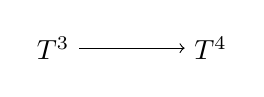
\begin{tikzpicture}[node distance=2cm]
	\node (t3) {$T^3$};
	\node[right of=t3] (t4) {$T^4$};
\draw[->] (t3) -- (t4);
\end{tikzpicture}

\begin{enumerate}[i)]
	\item
	Acyclic dependency graph
	$\Rightarrow$ conflict-serializable.

	Equivalent serial schedule:
	$T^1 \rightarrow T^2 \rightarrow T^3 \rightarrow T^4$.
\end{enumerate}

\item $S_3$:

Conflicting operations:
\begin{itemize}
	\item $r_2(w)$ before $w_1(w)$ on item $w$
	\item $w_3(x)$ before $w_2(x)$ on item $x$
	\item $w_2(x)$ before $w_4(x)$ on item $x$
	\item $w_2(y)$ before $w_5(y)$ on item $y$
	\item $r_1(v)$ before $w_5(v)$ on item $v$
	\item $w_5(v)$ before $w_4(v)$ on item $v$
\end{itemize}

Dependency graph $S_3$: \newline
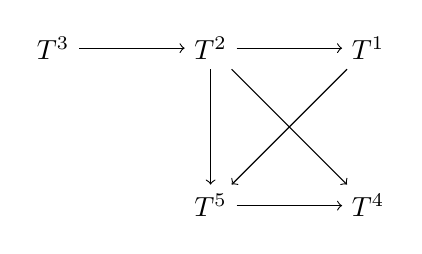
\begin{tikzpicture}[node distance=2cm]
	\node (t3) {$T^3$};
	\node[right of=t3] (t2) {$T^2$};
	\node[right of=t2] (t1) {$T^1$};
	\node[below of=t2] (t5) {$T^5$};
	\node[right of=t5] (t4) {$T^4$};

	\draw[->] (t3) -- (t2);
	\draw[->] (t2) -- (t1);
	\draw[->] (t2) -- (t5);
	\draw[->] (t1) -- (t5);
	\draw[->] (t2) -- (t4);
	\draw[->] (t5) -- (t4);
\end{tikzpicture}

\begin{enumerate}[i)]
	\item
	Acyclic dependency graph
	$\Rightarrow$ conflict-serializable.

	Equivalent serial schedule:
	$T^3 \rightarrow T^2 \rightarrow T^1 \rightarrow T^5 \rightarrow T^4$.
\end{enumerate}

\end{enumerate}
